%!TEX root = slides.tex

\section{Bayesian Logistic Regression}

\subsection{Recommended References}
\begin{frame}{Bayesian Logistic Regression - Recommended References}
    \begin{vfilleditems}
        \item \textcite{gelman2013bayesian} - Chapter 16: Generalized linear models
        \item \textcite{mcelreath2020statistical}:
        \begin{vfilleditems}
            \item Chapter 10: Big Entropy and the Generalized Linear Model
            \item Chapter 11, Section 11.1: Binomialregression
        \end{vfilleditems}
        \item \textcite{gelman2020regression}:
        \begin{vfilleditems}
            \item Chapter 13: Logistic regression
            \item Chapter 14: Working with logistic regression
            \item Chapter 15, Section 15.3: Logistic-binomial model
            \item Chapter 15, Section 15.4: Probit regression
        \end{vfilleditems}
    \end{vfilleditems}
\end{frame}

\subsection{Binary Data}
\begin{frame}{Binary Data\footnote{
            also known as dichotomous, dummy, indicator variable, etc.}
    }
    We use logistic regression when our dependent variable is \textbf{binary}.
    It only takes two distinct values,
    usually coded as $0$ and $1$.
\end{frame}

\subsection{What is Logistic Regression}
\begin{frame}{What is Logistic Regression}
    Logistic regression behaves exactly as a linear model:
    it makes a prediction by simply computing a weighted sum of the
    independent variables $\mathbf{X}$ using the estimated coefficients $\boldsymbol{\beta}$,
    along with a constant term $\alpha$.
    However, instead of outputting a continuous value $\mathbf{y}$,
    it returns the \textbf{logistic function} of this value:
    $$
        \text{logistic}(x) = \frac{1}{1 + e^{-x}}
    $$
\end{frame}


\subsubsection{Logistic Function}

\begin{frame}{Logistic Function}
    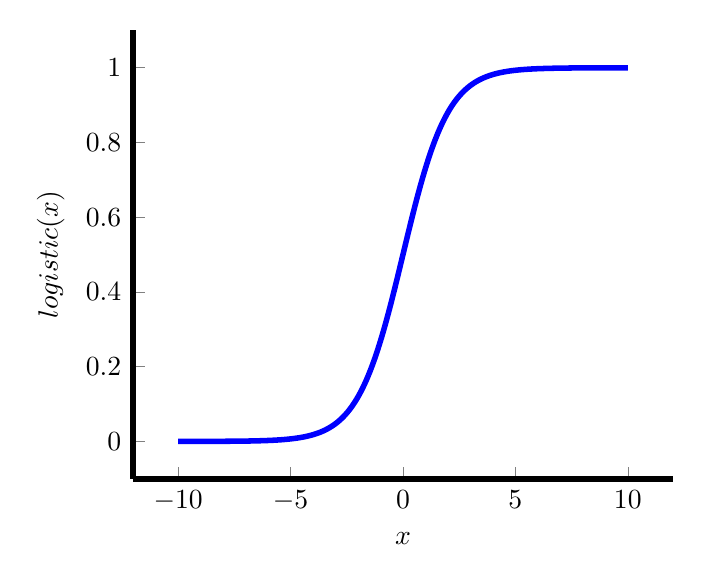
\begin{tikzpicture}
        \begin{axis}[every axis plot, line width=2pt,
                ylabel={$\text{logistic}(x)$},
                xlabel={$x$},
                domain=-10:10,samples=200,
                axis x line*=bottom, % no box around the plot, only x and y axis
                axis y line*=left % the * suppresses the arrow tips
            ]

            \addplot [blue] (x,{1/(1+exp(-x))});
        \end{axis}
    \end{tikzpicture}
\end{frame}

\subsubsection{Probit Function}
\begin{frame}{Probit Function}
    We can also opt to choose to use the \textbf{probit function}
    (usually represented by the Greek letter $\Phi$)
    which is the CDF of a normal distribution:
    $$
        \Phi (x)= \frac {1}{\sqrt {2 \pi}}\int _{-\infty }^{x}e^{-t^{2}/2}\,dt
    $$
\end{frame}

\begin{frame}{Probit Function}
    \begin{tikzpicture}
        \begin{axis}[every axis plot, line width=2pt,
                ylabel={$\Phi(x)$},
                xlabel={$x$},
                domain=-10:10,samples=200,
                axis x line*=bottom, % no box around the plot, only x and y axis
                axis y line*=left % the * suppresses the arrow tips
            ]

            \addplot [blue] {normcdf(0, 1)};
        \end{axis}
    \end{tikzpicture}
\end{frame}

\subsubsection{Logistic Function versus Probit Function}
\begin{frame}{Logistic Function versus Probit Function}
    \begin{tikzpicture}
        \begin{axis}[every axis plot, line width=1pt,
                ylabel={$f(x)$},
                xlabel={$x$},
                domain=-10:10,samples=200,
                axis x line*=bottom, % no box around the plot, only x and y axis
                axis y line*=left % the * suppresses the arrow tips
            ]
            \addplot [blue] (x,{1/(1+exp(-x))});
            \addlegendentry{logistic}
            \addplot [red] {normcdf(0, 1)};
            \addlegendentry{probit}
        \end{axis}
    \end{tikzpicture}
\end{frame}

\subsection{Comparison with Linear Regression}
\begin{frame}{Comparison with Linear Regression}
    Linear regression follows the following mathematical expression:
    \small
    $$
        \text{linear} = \alpha + \beta_1 x_1 + \beta_2 x_2 + \dots + \beta_k x_k
    $$
    \begin{vfilleditems}
        \item \small $\alpha$ -- intercept.
        \item \small $\boldsymbol{\beta} = \beta_1, \beta_2, \dots, \beta_k$ -- independent variables' $x_1, x_2, \dots, x_k$ coefficients.
        \item \small $k$ -- number of independent variables.
    \end{vfilleditems}
    If you implement a small mathematical transformation,
    you'll have \textbf{logistic regression}:
    \begin{vfilleditems}
        \item \small $\hat{p} = \text{logistic}(\text{linear}) = \frac{1}{1 + e^{-\operatorname{linear}}}$ --
        probability of an observation taking value $1$.
        \item \small $\hat{y} = \begin{cases} 0 & \text { if } \hat{p} < 0.5 \\ 1 & \text { if } \hat{p} \geq 0.5 \end{cases}$ --
        $\mathbf{y}$'s predicted binary value.
    \end{vfilleditems}
\end{frame}

\subsection{Logistic Regression Specification}
\begin{frame}{Logistic Regression Specification}
    We can model logistic regression using two approaches:
    \begin{vfilleditems}
        \item \textbf{Bernoulli likelihood} --
        \textbf{binary} dependent variable \textbf{y} which results from a
        Bernoulli trial with some probability $p$
        \item \textbf{binomial likelihood} --
        \textbf{discrete and positive} dependent variable $\textbf{y}$
        which results from $k$ successes in $n$ independent Bernoulli
        trials.
    \end{vfilleditems}
\end{frame}

\subsubsection{Bernoulli Likelihood}
\begin{frame}{Bernoulli Likelihood}
    \small
    $$
        \begin{aligned}
            \mathbf{y}         & \sim \text{Bernoulli}\left( p\right)                                      \\
            p                  & = \text{logistic/logit}(\alpha +  \mathbf{X} \boldsymbol{\beta})          \\
            \alpha             & \sim \text{Normal}(\mu_\alpha, \sigma_\alpha)                             \\
            \boldsymbol{\beta} & \sim \text{Normal}(\mu_{\boldsymbol{\beta}}, \sigma_{\boldsymbol{\beta}})
        \end{aligned}
    $$
    where:
    \begin{vfilleditems}
        \item \small $\mathbf{y}$ - \textbf{dependent binary variable}.
        \item \small $p$ - probability of $\mathbf{y}$ taking value of $1$ --
        success in an independent Bernoulli trial.
        \item \small $\text{logistic/logit}$ -- logistic or logit function.
        \item \small $\alpha$ -- intercept (also called constant).
        \item \small $\boldsymbol{\beta}$ -- coefficient vector.
        \item \small $\mathbf{X}$ -- data matrix.
    \end{vfilleditems}
\end{frame}

\subsubsection{Binomial Likelihood}
\begin{frame}{Binomial Likelihood}
    \small
    $$
        \begin{aligned}
            \mathbf{y}         & \sim \text{Binomial}\left(n,  p\right)                                    \\
            p                  & = \text{logistic/probit}(\alpha +  \mathbf{X} \boldsymbol{\beta})         \\
            \alpha             & \sim \text{Normal}(\mu_\alpha, \sigma_\alpha)                             \\
            \boldsymbol{\beta} & \sim \text{Normal}(\mu_{\boldsymbol{\beta}}, \sigma_{\boldsymbol{\beta}})
        \end{aligned}
    $$
    where:
    \begin{vfilleditems}
        \item \small $\mathbf{y}$ - \textbf{discrete positive variable} -- $k$ successes of $n$ independent Bernoulli trials.
        \item \small $n$ - number of independent Bernoulli trials.
        \item \small $p$ - probability of $\mathbf{y}$ taking value of $1$ --
        success in an independent Bernoulli trial.
        \item \small $\text{logistic/probit}$ -- logistic or probit function.
        \item \small $\alpha$ -- intercept (also called constant).
        \item \small $\boldsymbol{\beta}$ -- coefficient vector.
        \item \small $\mathbf{X}$ -- data matrix.
    \end{vfilleditems}
\end{frame}
\subsection{Bayesian Logistic Regression in Pumas}
\begin{frame}{Bayesian Logistic Regression in Pumas}
    \centering
    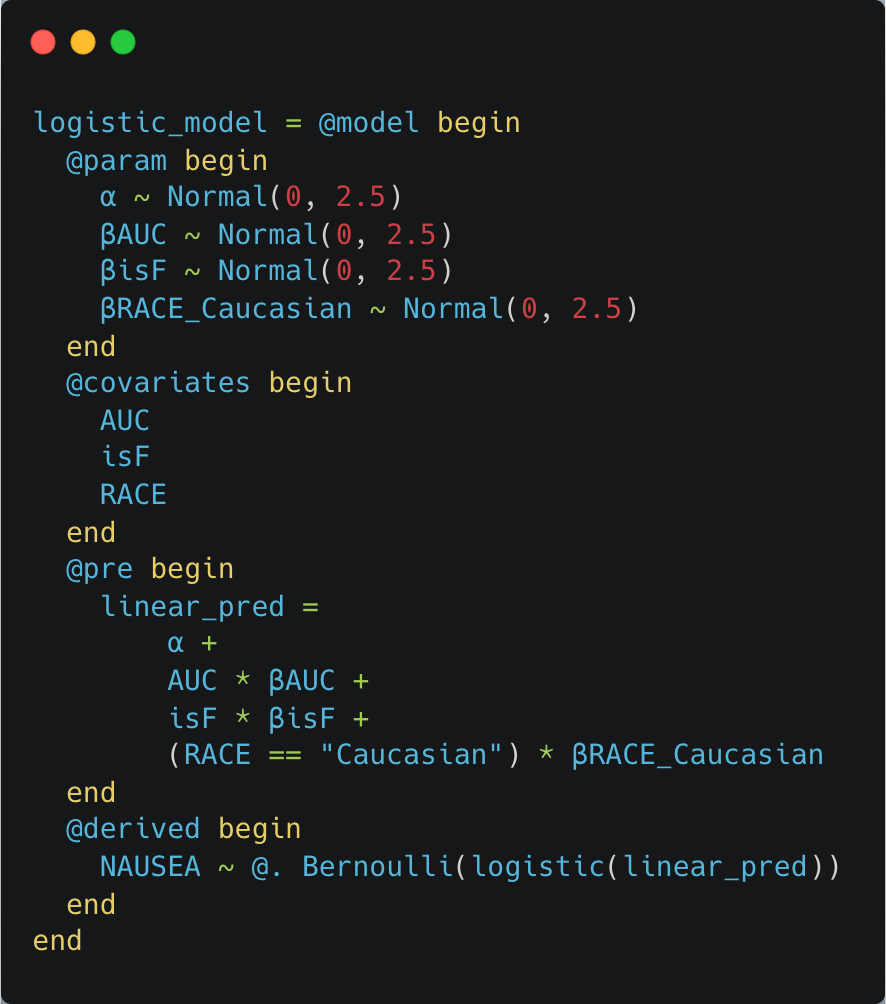
\includegraphics[width=0.4\columnwidth]{log_reg.png}
\end{frame}
